\section{Scattering and the LSZ Reduction Formula}

\subsection{Motivation}
We've focused on correlation functions to relate our theories to experiments. Now, we see how correlators enter into scattering - one of our most direct probes of nature.

Smashing things together can tell us a lot about systems; for example it can reveal the shape of composite particles, e.g. Rutherford scattering of electrons off of a nucleus. 

\begin{center}
    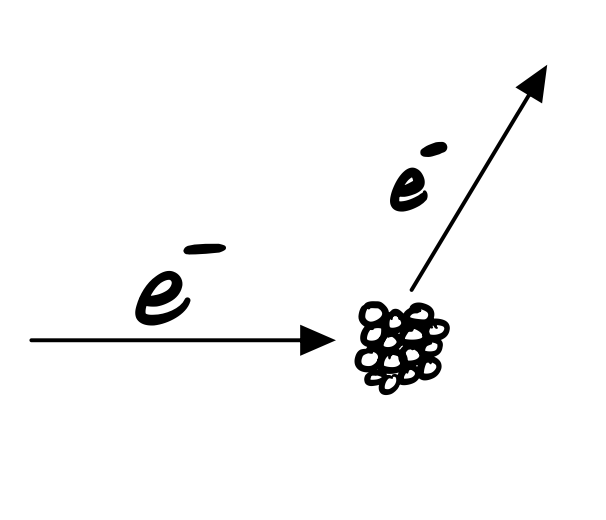
\includegraphics[scale=0.3]{Lectures/Figures/lec16-rutherford.png}
\end{center}

We can also probe the structure of interactions, e.g. a collision between an electron and proton, and even learn about the presence of other particles if we observe that there is energy missing/the scattering appears ``inelastic'' (e.g. on the left we have an elastic collision, on the right we have a collision that appears inelastic as at high enough energy, an unstable pion that decays into two photons is produced, and we didn't keep track of the energy of these).

\begin{center}
    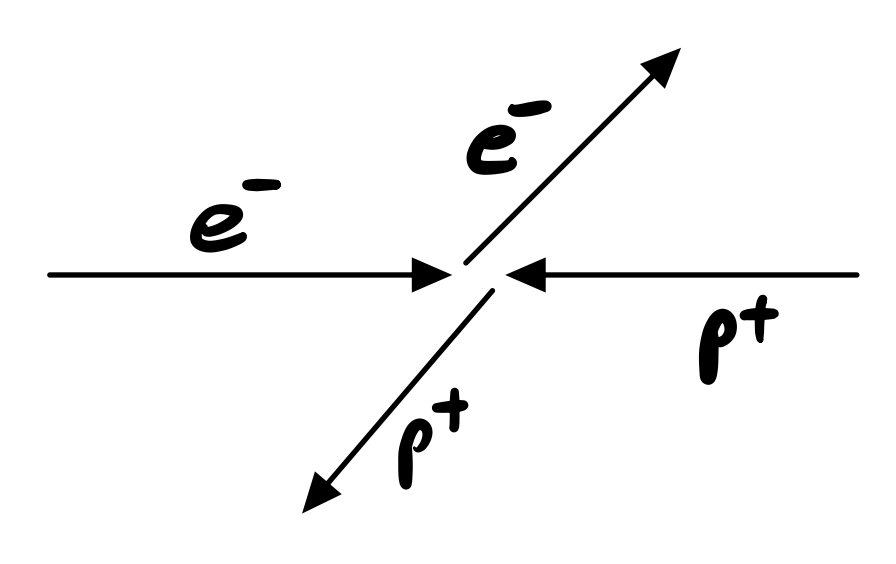
\includegraphics[scale=0.3]{Lectures/Figures/lec16-elasticcollision.png}
    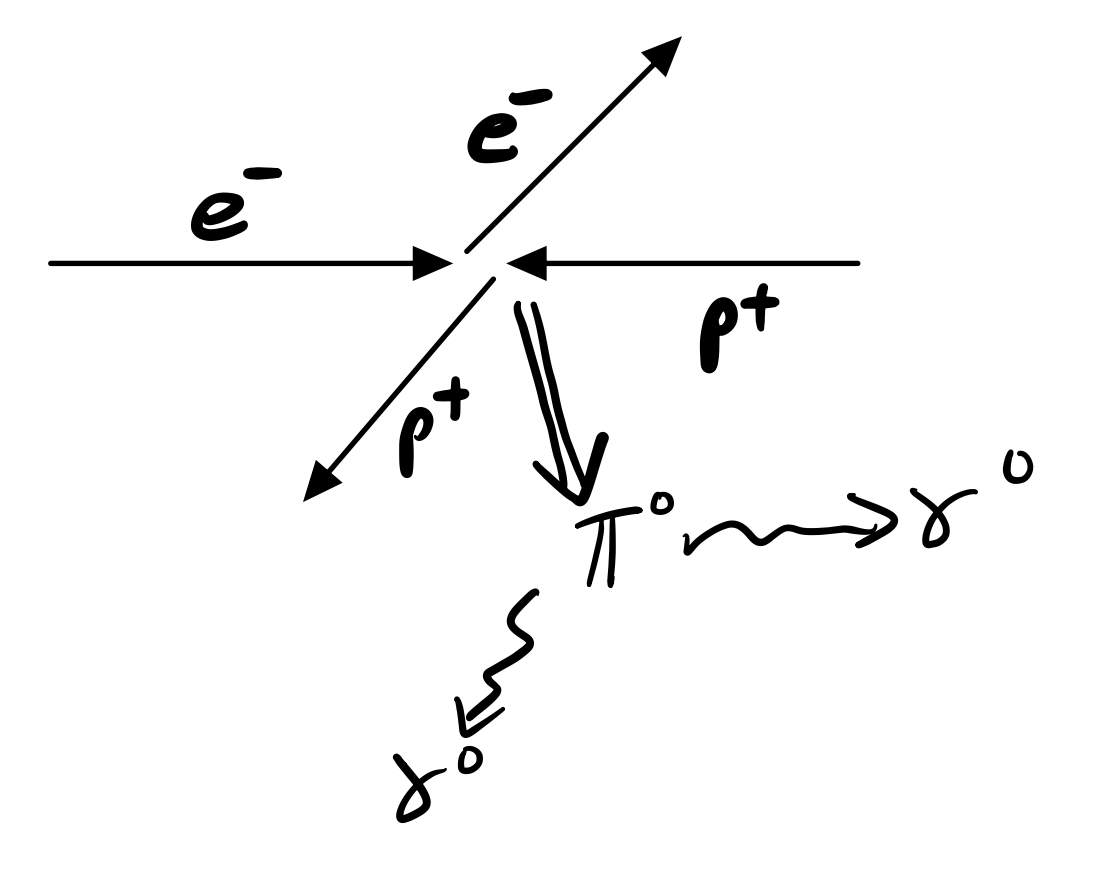
\includegraphics[scale=0.3]{Lectures/Figures/lec16-inelasticcollision.png}
\end{center}

What can we say about scattering states? Clearly, they have nontrivial time evolution and thus are not eigenstates. But, at $t \to -\infty$, they look like a collection of single-particle eigenstates. Let's take that as our starting point.

\subsection{Trivial time-evolution of free theories}

Recall single particle states for a free QFT. There, we have:
\begin{equation}
    \ket{\v{k}} = \hat{a}^\dag_{\v{k}}\ket{0}
\end{equation}
with the Lorentz-covariant normalization:
\begin{equation}
    \braket{\v{k}}{\v{k}'} = 2\e_\v{k}(2\pi)^d\delta^d(\v{k} - \v{k}')
\end{equation}
with dispersion $\e_\v{k} = \sqrt{\v{k}^2 + m^2}$. The raising/lowering operators we could wwrite in terms of the fields and their conjugate momenta:
\begin{equation}
    \begin{split}
        \hat{a}_\v{k} &= \e_\v{k}\hat{\phi}_\v{k} + i\hat{\pi}_\v{k} = \e_\v{k}\hat{\phi}_\v{k} + i\p_t\hat{\phi}_\v{k}
        \\ \hat{a}_\v{k}^\dag &= \e_\v{k}\hat{\phi}_{-\v{k}} - i\hat{\pi}_{-\v{k}} = \e_\v{k}\hat{\phi}_{-\v{k}} - i\p_t\hat{\phi}_{-\v{k}}
    \end{split}
\end{equation}
Thus, we can write the field operator as:
\begin{equation}
    \hat{\phi}_\v{k} = \frac{1}{2}(\hat{a}_\v{k} + \hat{a}^\dag_{-\v{k}})
\end{equation}
and this choice of basis was conveneint at it diagonalized the Hamiltonian, with:
\begin{equation}
    [\hat{H}, \hat{a}_\v{k}^\dag] = \e_\v{k}\hat{a}^\dag_\v{k}
\end{equation}
Studying the time-dependence:
\begin{equation}
    \begin{split}
        \hat{\phi}_\v{k}(t) &= \frac{1}{2\e_\v{k}}e^{i\hat{H}t}(\hat{a}_\v{k} + \hat{a}^\dag_{-\v{k}})e^{-i\hat{H}t}
        \\ &= \frac{1}{2\e_\v{k}}(e^{-i\e_\v{k}t}a_\v{k} + e^{i\e_\v{k}t}a_{-\v{k}}^\dag)
    \end{split}
\end{equation}
and:
\begin{equation}
    \p_t \hat{\phi}_\v{k}(t) = \frac{i}{2}(e^{-i\e_\v{k}t}a_{\v{k}} - e^{i\e_\v{k}t}a_{-\v{k}}^\dag)
\end{equation}
Note then that:
\begin{equation}
    e^{-i\e_\v{k}t}a_\v{k} = (\e_\v{k} + i\p_t)\hat{\phi}_\v{k}(t) \implies a_\v{k} = e^{i\e_\v{k}}(\e_\v{k} + i\p_t)\hat{\phi}_\v{k}(t)
\end{equation}
is time-independent. The $\hat{a}_\v{k}$ creates a single particle state. We can create 2-particle (and more) states by acting via multiple raising operators $\ket{\v{k}_1 \ldots \v{k}_n} = a_{\v{k}_1}^\dag \ldots a_{\v{k}_n}^\dag\ket{0}$ but not much will happen in a free theory, the time dependence is trivial.

\subsection{Interacting theories - In/Out states and the S-Matrix}
The fact that the above expression for $\hat{a}_\v{k}$ was time-independent relied on the fact that $[\hat{H}, \hat{a}_\v{k}] = -\e_\v{k}\hat{a}_\v{k}$. But, with interactions the Hamiltonian generally has more terms than just the quadratic $\hat{a}^\dag\hat{a}$ term, and could have quartic (or higher) interactions. So, this time-independent expression does not generically hold; instead, they are time-dependent. However, we can still consider the expressions:
\begin{equation}
    \begin{split}
        a_\v{k}(t) &= e^{i\e_\v{k}}(\e_\v{k} + i\p_t)\hat{\phi}_\v{k}(t)
        \\ a_\v{k}^\dag(t) &= e^{-i\e_\v{k}}(\e_\v{k} - i\p_t)\hat{\phi}_{-\v{k}}(t)
    \end{split}
\end{equation}
Which we note are \emph{not} equal to the Heisenberg evolved operators $e^{i\hat{H}t}\hat{a}e^{-i\hat{H}t}$ in the interacting theory, as there will now be additional commutations of $\hat{a}$ with $\hat{H}$.

A guess for what creates a 2-particle state at asymptotically early times is:
\begin{equation}
    \ket{i} = a_{\v{k}_1}^\dag(t=-\infty)a_{\v{k}_2}^\dag(t=-\infty)\ket{0}
\end{equation}
i.e. we assume that in the infinite past, we just have these simple 2-particle states as we did in the free theory. The intuition for this is far-separated wavepackets do not interact. Note that however these are not 2-particle eigenstates in the interacting theory. But this is OK. All that we need for this to work is for objects like $a^\dag_{\v{k}_1}(-\infty)\ket{0}$ to have some overlap with the true single-particle eigenstates of the interacting Hamiltonian/theory, $\bra{\v{k}}$. I.e. we want:
\begin{equation}
    \bra{\v{k}}a^\dag_{\v{k}'}\ket{0} = C\delta^d(\v{k} - \v{k}')
\end{equation}
Note that we can't solve the interacting theory fully, but we do rely on the assumption that theories with a mass gap have well-defined single-particle excitations. Also note that the fact that the above overlap is proportional to a delta function follows by spatial translation symmetry.

So, we have a candidate for the ``in'' states to scattering. Now, let's consider the ``out'' states. Even though there may be very very complicated dynamics and states at intermediate times, the ``out'' states can be assumed to also be very simple at late times:
\begin{equation}
    \ket{f} = a^\dag_{\v{k}_1'}(t=+\infty)a^\dag_{\v{k}_2'}(t=+\infty)\ket{0}
\end{equation}
Note that if we reverse time evolve an out state back to very early times we will have something that looks very complicated (and same for the in states - if we time evolve it it will be a complicated linear combination of out states). Note also - we consider exact $\v{k}$ states here, in reality Heisenberg uncertainty tells us that we should consider smeared wavepackets. It doesn't change the discussion that much, so for our discussion here we ignore it (but if you read Srednicki, you will see the smearing go along for the ride there).

The ``S-Matrix'' is the amplitude for a specific ``in'' state $\ket{i}$ to, after time evolution, produce a given out state $\ket{f}$:
\begin{equation}
    S_{fi} = \braket{f}{i}
\end{equation}
with:
\begin{equation}
    p(i \to f) = \abs{\braket{f}{i}}^2
\end{equation}
One might worry that there doesn't appear to be time-evolution appearing in the above expression (we take the direct overlap of $\ket{i}$ and $\ket{f}$), but the time-evolution is in some sense accounted for in $\ket{f}$, and this definition of the matrix elements does indeed give the relevant amplitudes.

\subsection{2-to-2 S-matrix and LSZ formula}
Consider the matrix elements for a 2 particle to 2 particle scattering:
\begin{equation}
    \braket{f}{i} = \bra{0}\hat{a}_{\v{k}_1'}(\infty)\hat{a}_{\v{k}_2'}(\infty)\hat{a}_{\v{k}_1}(-\infty)\hat{a}_{\v{k}_2}(-\infty)\ket{0}
\end{equation}
We start by finding a formula for the difference $\hat{a}_\v{k}^\dag(\infty) - \hat{a}_\v{k}^\dag(-\infty)$, which would vanish in the free theory.

We write the difference as an integral over time:
\begin{equation}
    \begin{split}
        \hat{a}^\dag_\v{k}(\infty) - \hat{a}_\v{k}^\dag(-\infty) &= \int_{-\infty}^\infty dt \p_t \hat{a}^\dag_\v{k}(t) 
        \\ &= \int_{-\infty}^\infty dt \p_t\left[e^{-i\e_\v{k}t}(\e_\v{k} - i\p_t)\hat{\phi}_{-\v{k}}(t)\right]
        \\ &=\int dt e^{-i\e_\v{k}t}(-i\e_\v{k} + \p_t)(-i)(i\e_\v{k} + \p_t)\hat{\phi}_{-\v{k}}(t)
        \\ &= -i\int dt e^{-i\e_\v{k}t}(\p_t^2 + k^2 + m^2)\hat{\phi}_{-\v{k}}(t)
    \end{split}
\end{equation}
Now plugging in the Fourier transform of the $\hat{\phi}_{-\v{k}}  \int d^dx e^{i\v{k} \cdot \v{x}}\hat{\phi}(t, \v{x})$:
\begin{equation}
    \hat{a}^\dag_\v{k}(\infty) - \hat{a}_\v{k}^\dag(-\infty) = -i\int d^{d+1}x e^{-i\e_\v{k}t + i\v{k} \cdot \v{x}}(\p_t^2 + k^2 + m^2)\hat{\phi}(t, \v{x})
\end{equation}
Now, we observe that the $k^2$ is the same thing as the $-\nabla^2$ acting on the left (brings down two factors of $(i\v{k})$). By twicefold integration by parts, we can make it act on the right, and so:
\begin{equation}
    \hat{a}^\dag_\v{k}(\infty) - \hat{a}_\v{k}^\dag(-\infty) = -i\int d^{d+1}x e^{-i\e_\v{k}t + i\v{k} \cdot \v{x}}\left(\p_t^2 - \nabla^2 + m^2\right)\hat{\phi}(t, \v{x})
\end{equation}
Thus:
\begin{equation}
    \boxed{\hat{a}^\dag_\v{k}(\infty) - \hat{a}_\v{k}^\dag(-\infty) = -i\int d^{d+1}x e^{ik_\mu k^\mu}(m^2 - \p^2)\hat{\phi}(t, \v{x})}
\end{equation}
with $k_\mu = (-\e_\v{k}, \v{k})$. We notice that the $\p^2 - m^2$ operator is just the Klein-Gordon operator, for which $(\p^2-m^2)\phi = 0$ in a free theory, as we said it would. But it does \emph{not} vanish in an interacting theory. For example with $\mathcal{L}_{\text{int}} = \frac{1}{3}\lambda \phi^3$ we would get something like:
\begin{equation}
    (\p^2 - m^2)\phi = \lambda \phi^2 \neq 0
\end{equation}

The expression we derived looks somewhat complicated, but it will eventually simplify a lot, when we plug it into our expression into $\braket{f}{i}$. Before doing so, we add in the time-ordering symbol for free:
\begin{equation}
    \braket{f}{i} = \bra{0}\mathcal{T}\{\hat{a}_{\v{k}_1'}(\infty)\hat{a}_{\v{k}_2'}(\infty)\hat{a}_{\v{k}_1}(-\infty)\hat{a}_{\v{k}_2}(-\infty)\}\ket{0}
\end{equation}
Then, using what we have derived for the difference, we can write:
\begin{equation}
    \begin{split}
        \hat{a}^\dag_{\v{k}_1}(-\infty) = a_{\v{k}_1}^\dag(\infty) + i\int_{x_1}e^{ik_1x_1}(m^2 - \p_{x_1}^2)\phi(x_1)
        \\ \hat{a}_{\v{k}'_1}(\infty) = a_{\v{k}_1}(-\infty) + i\int_{x_1'}e^{-ik_1x_1'}(m^2 - \p_{x_1'}^2)\phi(x_1')
    \end{split}
\end{equation}
Thanks to the time-ordering (which interachanges the order of things such that we get annihilations of the vaccum via $a\ket{0} = 0$ and $\bra{0}a^\dag = 0$), we end up with:
\begin{equation}
    \boxed{\braket{f}{i} = i^4\int_{x_1x_2x_1'x_2'}e^{ik_1x_1}e^{ik_2x_2}e^{-ik_1'x_1'}e^{-ik_2'x_2'}(m^2 - \p_{x_1}^2)(m^2 - \p_{x_2}^2)(m^2 - \p_{x_1'}^2)(m^2 - \p_{x_2'}^2)\bra{0}\mathcal{T}\{\hat{\phi}(x_1)\hat{\phi}(x_2)\hat{\phi}(x_1')\hat{\phi}(x_2')\}\ket{0}}
\end{equation}
This is the LSZ-formula for 2-to-2 scattering. But it can be easily generalized to $n$-to-$n'$ (see Srednicki Eq. (5.15) - there we see that we get a $n + n'$-point function). But the most experimentally relevant ones will be $2$-to-$n'$.

The key takeaway is that the S-matrix is basically made up of time-ordered correlators.

\subsection{2 Comments - Normalization and (No) Multiple Particles}
There is one slight subtlety here. In an interacting theory, we generically expect that our normalization coefficient $C$ will not be unity;
\begin{equation}
    \bra{\v{k}}a_{\v{k}'}^\dag\ket{0} = C\delta(\v{k} - \v{k}')
\end{equation}
Said differently:
\begin{equation}
    \bra{\v{k}}\hat{\phi}(\v{x})\ket{0} = \bra{\v{k}}e^{i\v{P} \cdot \v{x}}\phi(0)e^{-i\v{P}\cdot\v{x}}\ket{0} = e^{i\v{k}\cdot\v{x}}\bra{\v{k}}\phi(0)\ket{0}
\end{equation}
The $\bra{\v{k}}\phi(0)\ket{0}$ is a Lorentz scalar, and the $k$-dependence can only enter through $k^2 = -m^2$. Thus it depends on the parameters of the theory $(\lambda, \lambda', m^2, \ldots)$. For free theory, $\bra{\v{k}}\phi(0)\ket{0} = 1$. We will now rescale $\hat{\phi}$ such that it is equal to one. In practice, this is accomplished via adding $-\frac{1}{2}\delta Z\int (\p\phi)^2$ to the Lagrangian.

Furthermore, one can check that $a^\dag_{\v{k}}(-\infty)$ does \emph{not} create multi-particle states (at asymptotically early times). The detailed argument is given in Srednicki Section 5 (read it!) but here we give the intuition. Namely, it does not have the correct energy to create multiple particles - this observation crucially relies on a mass gap, or separation between single-particle states and the rest of the spectrum, as is sketched below:

\begin{center}
    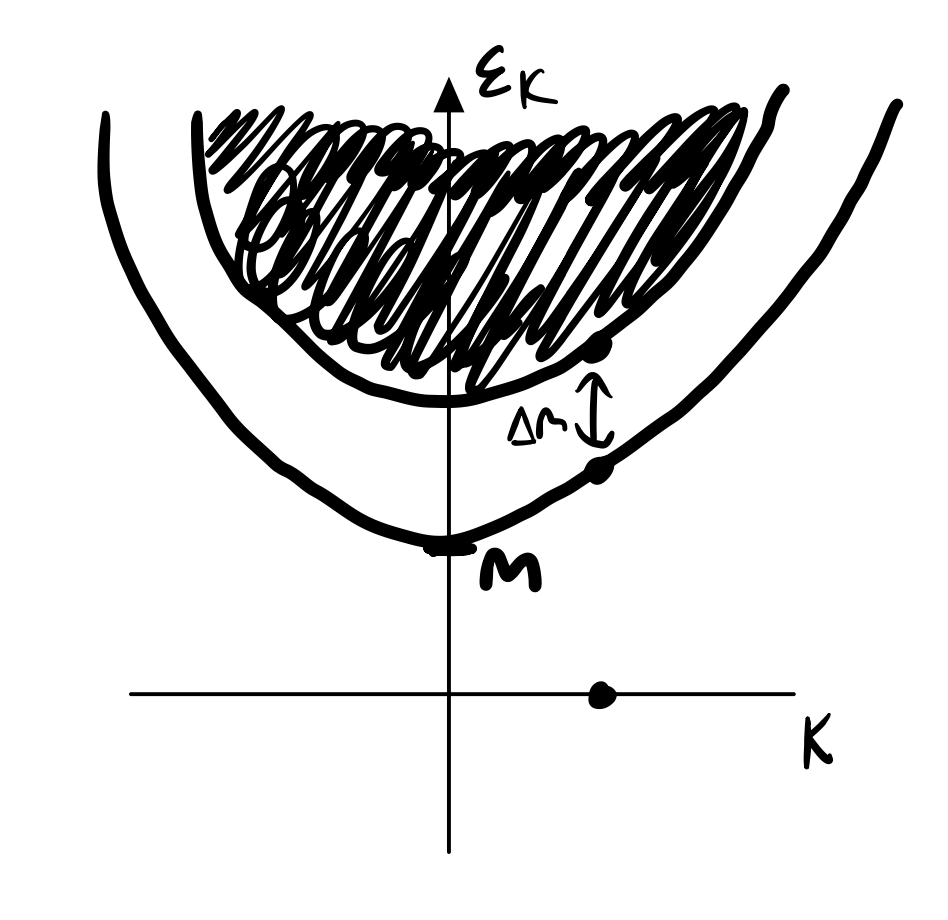
\includegraphics[scale=0.3]{Lectures/Figures/lec16-massgap.png}
\end{center}

This tells us that it is not possible for define the S-matrix for massless/gapless theories. Unfortunately, this contains QFTs that we see in nature, including Conformal Field Theories/CFTs. These issues can be tackled in QED using techniques of soft divergence. But for strongly interacting gapless theories, we can't distinguish single-particle states from a soup of dressed multiple particles, and there is no hope for the S-matrix.